\scanpage{31}
\reversemarginpar
\margin{\figure{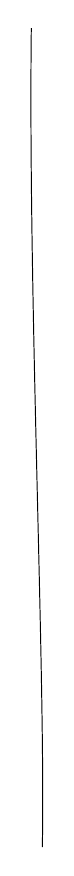
\begin{tikzpicture}[x=1cm,y=1cm]
\draw[line width=.35pt] (0,-.4) .. controls (-.04,-3.8) and (.18,-8.6) .. (.14,-10.8);
\end{tikzpicture}}}
\normalmarginpar
\uline{Théorème} 2.1.1. Soit $f:S'\handwritten{\longrightarrow}S$ un morphisme universellement localement \uline{$L$}-\unsure{1|l}-asphérique (SGA 4 XV \handwritten{1.11}), par exemple (SGA\handwritten{4}XV \handwritten{2.1}) un morphis\unsure{me} lisse, ou tel que $\deleted{\unsure{X}}\handwritten{S'}$ soit isomorphe à la limite\inserted{projective} d'un systême projectif\inserted{filtrant} de $S$-schémas lisses $S'_i$ à morphismes de transition affines\deleted{\unsure{,}} (SGA 4 XV \handwritten{1.13\inserted{(ii)}})

Soi\inserted{en}t $g:X\handwritten{\longrightarrow}S$ un morphisme de schémas, d'où un carré car\deleted{\unsure{ét|té}}\unsure{té|ét}sien
\diagram{\begin{tikzcd}[
ampersand replacement=\&,column sep=2cm,row sep={1.2cm,between origins},
execute at end picture={
\draw[line width=.3pt] ([xshift=-.46cm,yshift=.40cm]s031ll.center) -- ([xshift=-.43cm,yshift=.17cm]s031ll.center);
\draw[line width=.3pt] ([xshift=-.29cm,yshift=.24cm]s031ll.center) .. controls ([xshift=-.25cm,yshift=.08cm]s031ll.center) and ([xshift=-.25cm,yshift=-.03cm]s031ll.center) .. ([xshift=-.29cm,yshift=-.11cm]s031ll.center);
}]
X \handwritten{\arrow[d]} \arrow[d,phantom,"g"'] \& X' \handwritten{\arrow[l]} \arrow[l,phantom,"f'"'] \handwritten{\arrow[d]} \arrow[d,phantom,"g'"] \\
|[alias=s031ll]| S \& S'\handwritten{\arrow[l]}\arrow[l,phantom,"f"']\rlap{,} \\[.1cm]
\inserted{\handwritten{(\overline{\text{\uline{V}}}\ 5\quad)}}\handwritten{,} \&
\end{tikzcd}}

$G$ un\inserted{ind-$L$-} champ sur $X$ \deleted{dont les faisceaux d'automorphismes sont des ind-\uline{$L$}-faisceaux} $G'=f'^{\handwritten{*}}(G)$ le champ image inverse sur $X'$.

\begin{enumerate}[label=\alph*)]
\item Si \deleted{$S$ et $S'$ sont strictement locaux et} $f$ est un morphisme \deleted{strictement} \uline{local} de schémas strictement locaux, alors le foncteur
\[
\handwritten{G(X)\longrightarrow G'(X')}
\]
est une équivalence de catégories.

\item Si $g$ est cohérent(i.e. quasi-compact et quasi-séparé) alors le morphisme de champs ``de changement de base''
\[
f^{\handwritten{'}}(g_{\handwritten{*}}(G))\handwritten{\longrightarrow}g'_{\handwritten{*}}(f'^{\handwritten{*}}(G))\deleted{\handwritten{\unsure{=g_*|g_*}}}
\]
est une équivalence de champs sur $S'$.
\end{enumerate}

\reversemarginpar
\margin{\figure{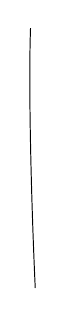
\begin{tikzpicture}[x=1cm,y=1cm]
\draw[line width=.35pt] (0,-.35) .. controls (-.03,-1.2) and (.02,-2.8) .. (.06,-3.65);
\end{tikzpicture}}}
\normalmarginpar
\uline{Corollaire} 2.1.2. Soient $k$ un corps séparablement clos, $k'$ une extension séparablement close de $k$, $X$ un $k$-schéma, $X'=X\handwritten{\otimes}_k k'$, alors pour tou\unsure{t} \deleted{champ $G$} ind-\uline{$L$}-champ $G$ sur $X$, désignant par $G'$ son image inverse sur $X'$, le foncteur
\[
\handwritten{G(X)\longrightarrow G'(X')}
\]
est une équivalence de catégories.

O\unsure{\(\mathbb{n}\)|\deleted{p}n|\deleted{n}p} sait en effet (SGA 4 XVI\quad\quad) que $\operatorname{Spec}(k')\handwritten{\longrightarrow}\operatorname{Spec}(k)$ est universellement localement \uline{$L$}-1-asphérique.

Démonstration. On prouve a) par référence à SGA 4 XVI (nouvelle édition !)\inserted{\handwritten{et à $\overline{\text{\uline{V}}}$ - -}}, et b) en se ramenant à a) par des lemmes 2.1.7.2 et 2.1.7.4 renumérotés.
% Bottom marginal addition, beginning beside the end of the preceding typed line.
\begin{flushright}\begin{minipage}{.68\linewidth}
\handwritten{En tout, ça devrait faire 3 pages au Ch.p $\overline{\text{\uline{VII}}}$ au maximum, -- mais il y aura renvois au Ch.p $\overline{\text{\uline{\unsure{V|I}}}}$.}
\end{minipage}\end{flushright}
% archive sheet number: 30
